\section{Authentication}
\label{design:authentication}
\subsection{Requirements}
\label{design:authentication:requirements}

\noindent Authentication consists of two steps:
\begin{enumerate}
	\item Validating
	\item Confirmation
\end{enumerate}
These steps are required to have in order to make authentication successful. The need for validation is to ensure privacy. Confirmation is a requirement as error prevention, incase of validation with wrong identity.
\subsection{Solution}
\label{design:authentication:solution}
Being able to launch a \girafapp[] as a specific guardian requires the user to interact such that the launcher knows which guardian the user represents.

As stated in \autoref{design:authentication:requirements}, privacy is required since: each modulated child and guardian contains private data and therefore needs to be protected.
QR-codes was chosen as means of authentication, as they provide a level of security.
An alternative to QR-codes could be a \emph{username-password} method, where each user have their own username, with an private password.
The launcher is developed towards being a tool usable by both guardians and children e.g. the ``child mode'' feature, described in \autoref{backlog:child_mode}.
A username-password combination requires the user to remember their credentials, whereas some \autists[] have problems with it.

\begin{quotation}
Some \autists[] can have problems remembering a username and password\\ 
	\begin{flushright}
		- Drazenko Banjak, educator at Egebakken.
	\end{flushright}
\end{quotation}

QR-codes provides a physical way of storing the user credentials and allows for other users to take responsibility of the QR-code, such as a \guardian[] carrying a QR-code of a \autist[].
They can be scanned by a built-in camera on tablets and can be printed using standard paper and printer equipment. 
They can be copied, by e.g. a copy machine, and therefore must be kept away from untrusted users, if they should not be used by people for which they were not intended.
To sum up, QR-codes are chosen because of they improve usability, despite of their ability to be copied.  \\\todo{Ulrik, er dette i orden? Bullet points plox}

This leads to the functionality solution seen in \autoref{fig:authentication_design}.
\begin{figure}[h]
	\centering
	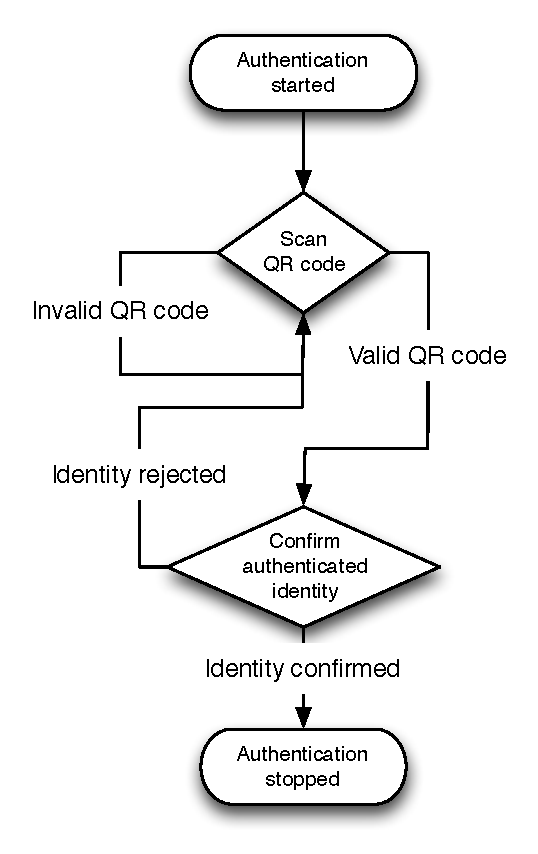
\includegraphics[width=0.5\textwidth]{gfx/authentication_design.pdf}
	%\caption{Features of the Authentication feature}
	\caption{Flowchart of the authentication functionality}
	\label{fig:authentication_design}
\end{figure}

Upon scanning a QR-code, there is two possible outcomes: The QR-code is invalid, as the credentials are not recognized, or the QR-code contains credentials which are recognized.
In case of the QR-code being valid, the process then enters it second step. The second step consist of the user needs to confirm the identity, or reject if identity represented on the system does not match the user's identity.

\subsubsection{GUI}
The GUI components of the authentication design, can be seen in \autoref{fig:authentication_gui_design_init}.
\begin{figure}[h]
	\centering
	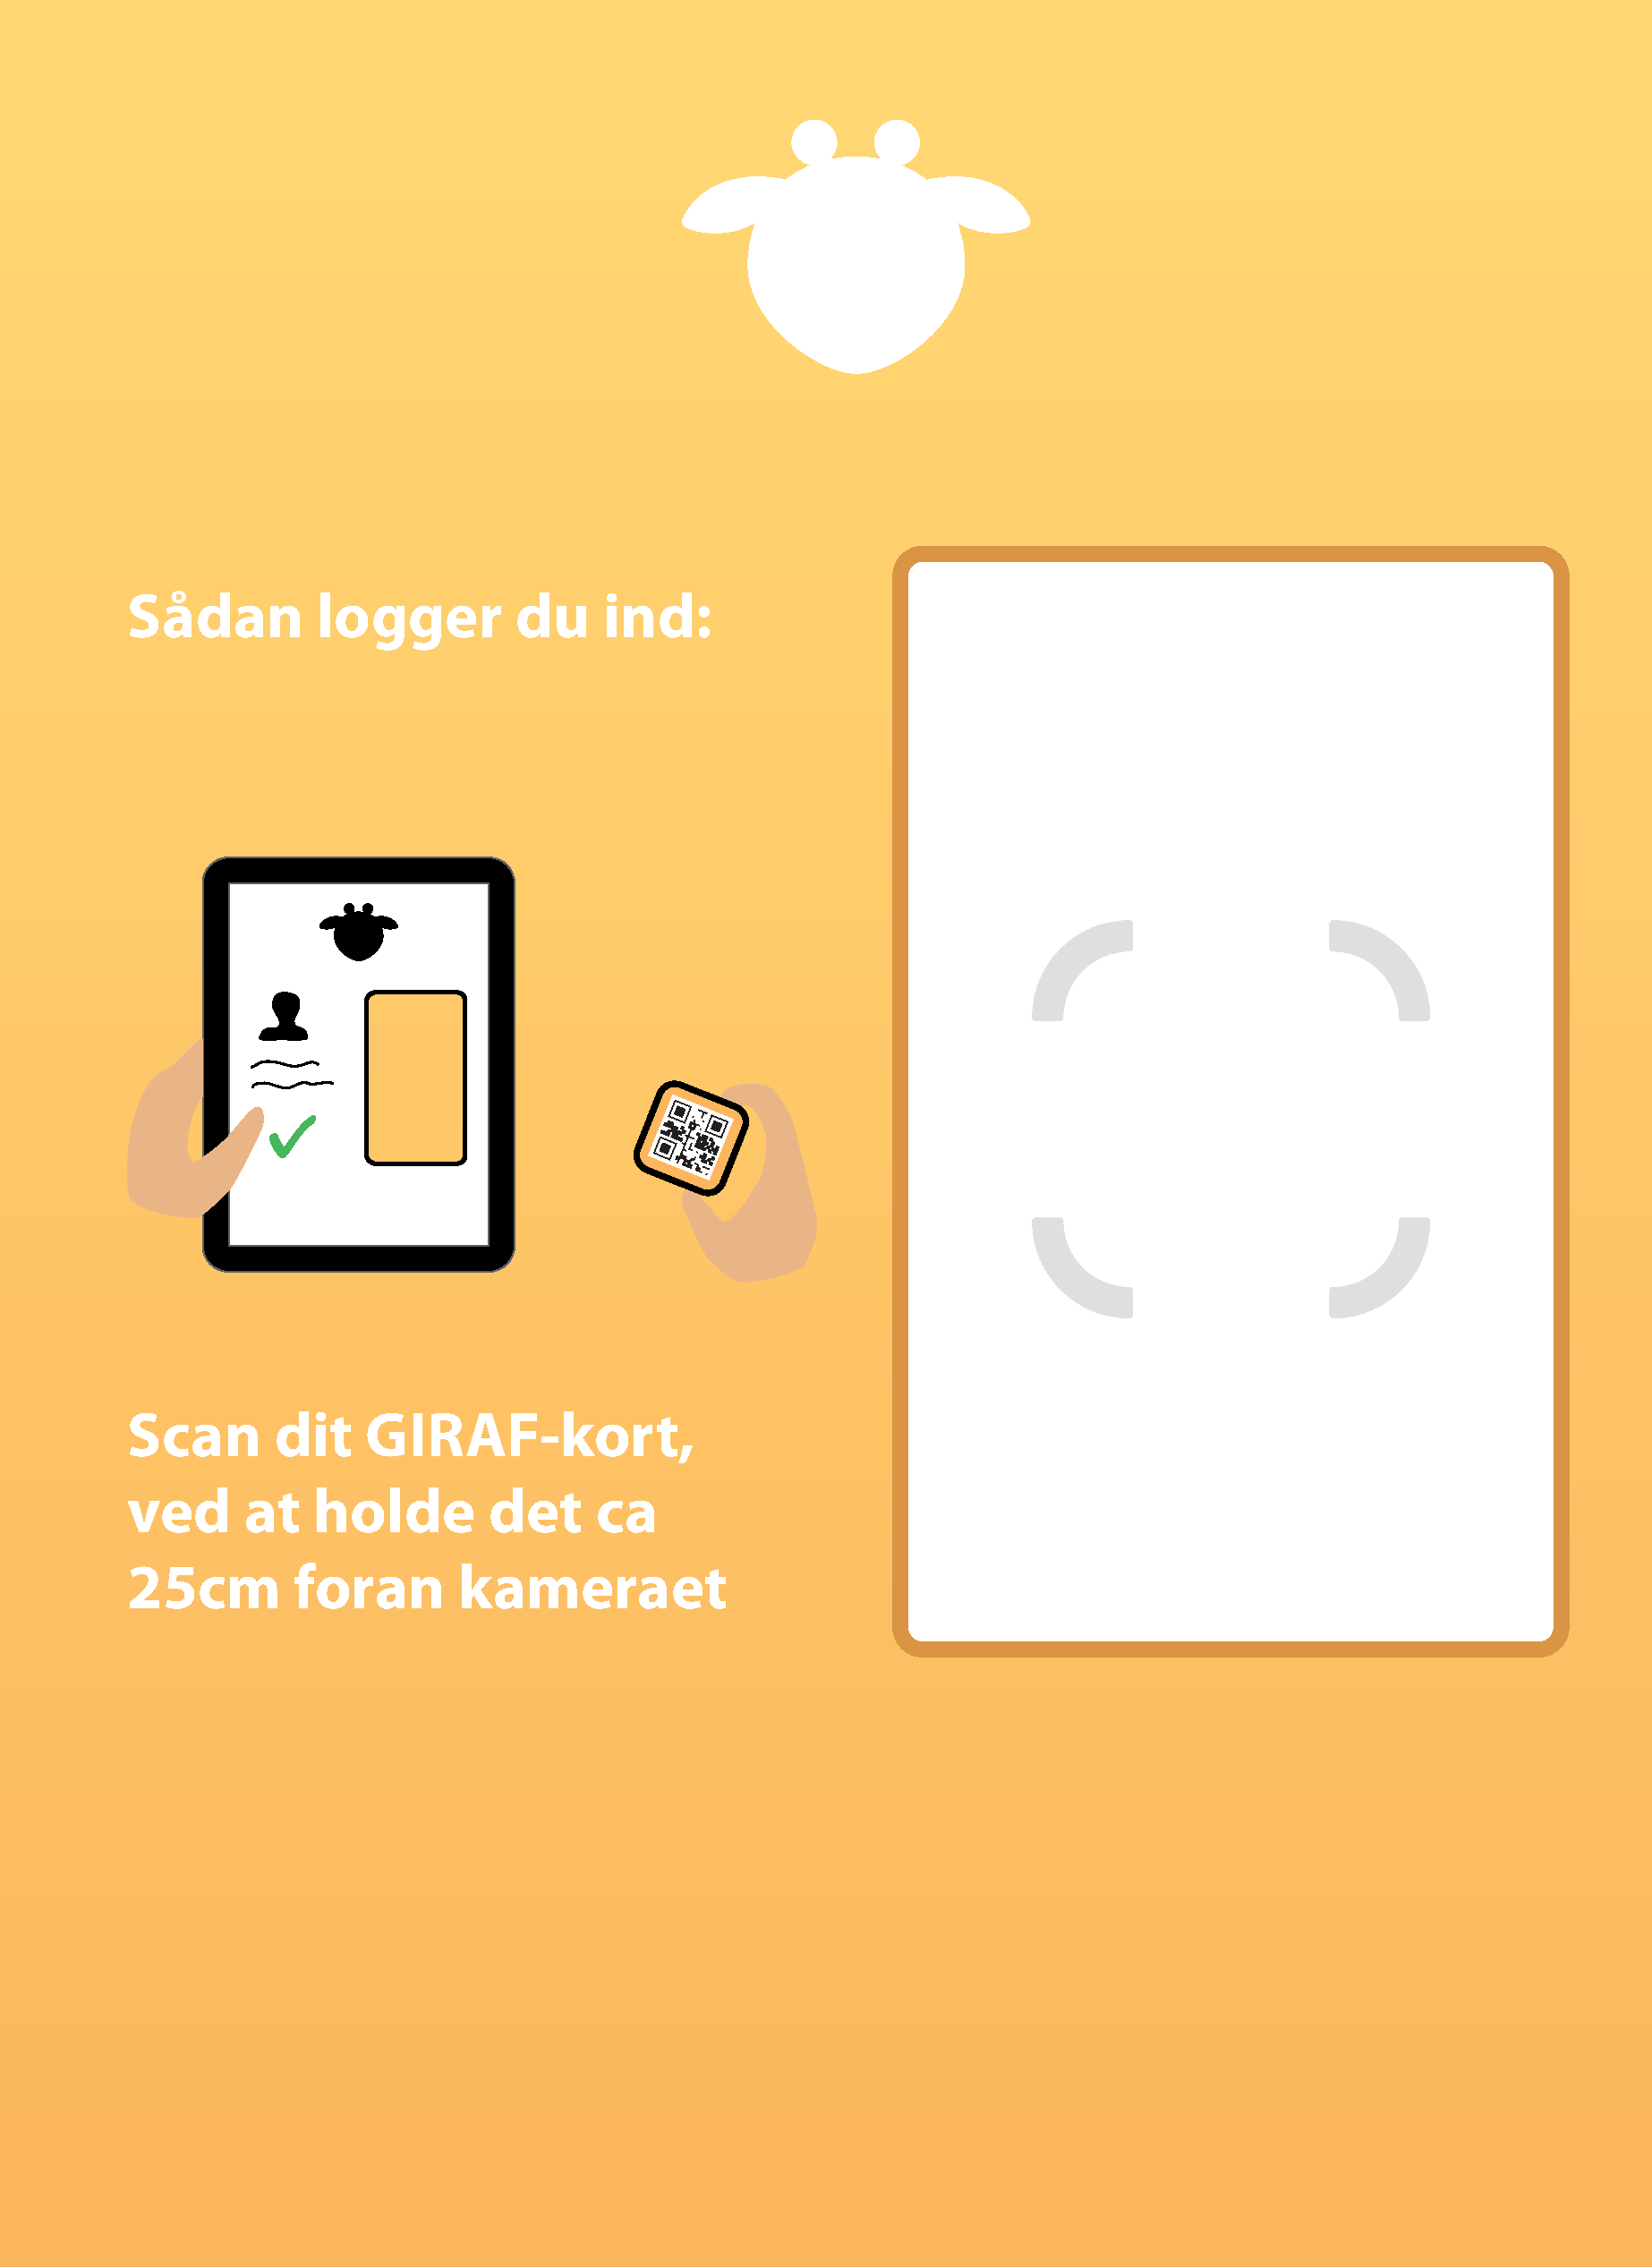
\includegraphics[width=0.7\textwidth]{gfx/authentication_gui_design_init.pdf}
	\caption{Graphical User Interface of the authentication functionality}
	\label{fig:authentication_gui_design_init}
\end{figure}
The camera border helps distinct the camera feed from the rest of the layout, but it also provides feedback upon scanning. 